% Created 2022-02-16 Wed 15:44
% Intended LaTeX compiler: pdflatex
\documentclass[11pt]{article}
\usepackage[utf8]{inputenc}
\usepackage[T1]{fontenc}
\usepackage{graphicx}
\usepackage{grffile}
\usepackage{longtable}
\usepackage{wrapfig}
\usepackage{rotating}
\usepackage[normalem]{ulem}
\usepackage{amsmath}
\usepackage{textcomp}
\usepackage{amssymb}
\usepackage{capt-of}
\usepackage{hyperref}
\usepackage{minted}
\author{Karthik Kumar}
\date{\today}
\title{}
\hypersetup{
 pdfauthor={Karthik Kumar},
 pdftitle={},
 pdfkeywords={},
 pdfsubject={},
 pdfcreator={Emacs 27.1 (Org mode 9.3)}, 
 pdflang={English}}
\begin{document}

\tableofcontents

\section{Distant measures}
\label{sec:org29f65a4}
Various types of distance measures and implementations

\section{Introduction}
\label{sec:orgceba741}
A distance measure is simply a means of calculation between two points
or objects. Distance measures are useful in identifying patterns in the
input data. Also, it can be used to recognize similarities among the
data.

\subsection{Euclidean Distance}
\label{sec:orgeb3936b}
The \textbf{Euclidean distance} between two points in Euclidean space is the
length of a line segment between the two points. It can be calculated
from the cartesian coordinates of the points using the Pythagorean
theorem. Euclidean distance works great when you have low-dimensional
data and the magnitude of the vectors is important to be measured.\\

\begin{figure}[htbp]
\centering
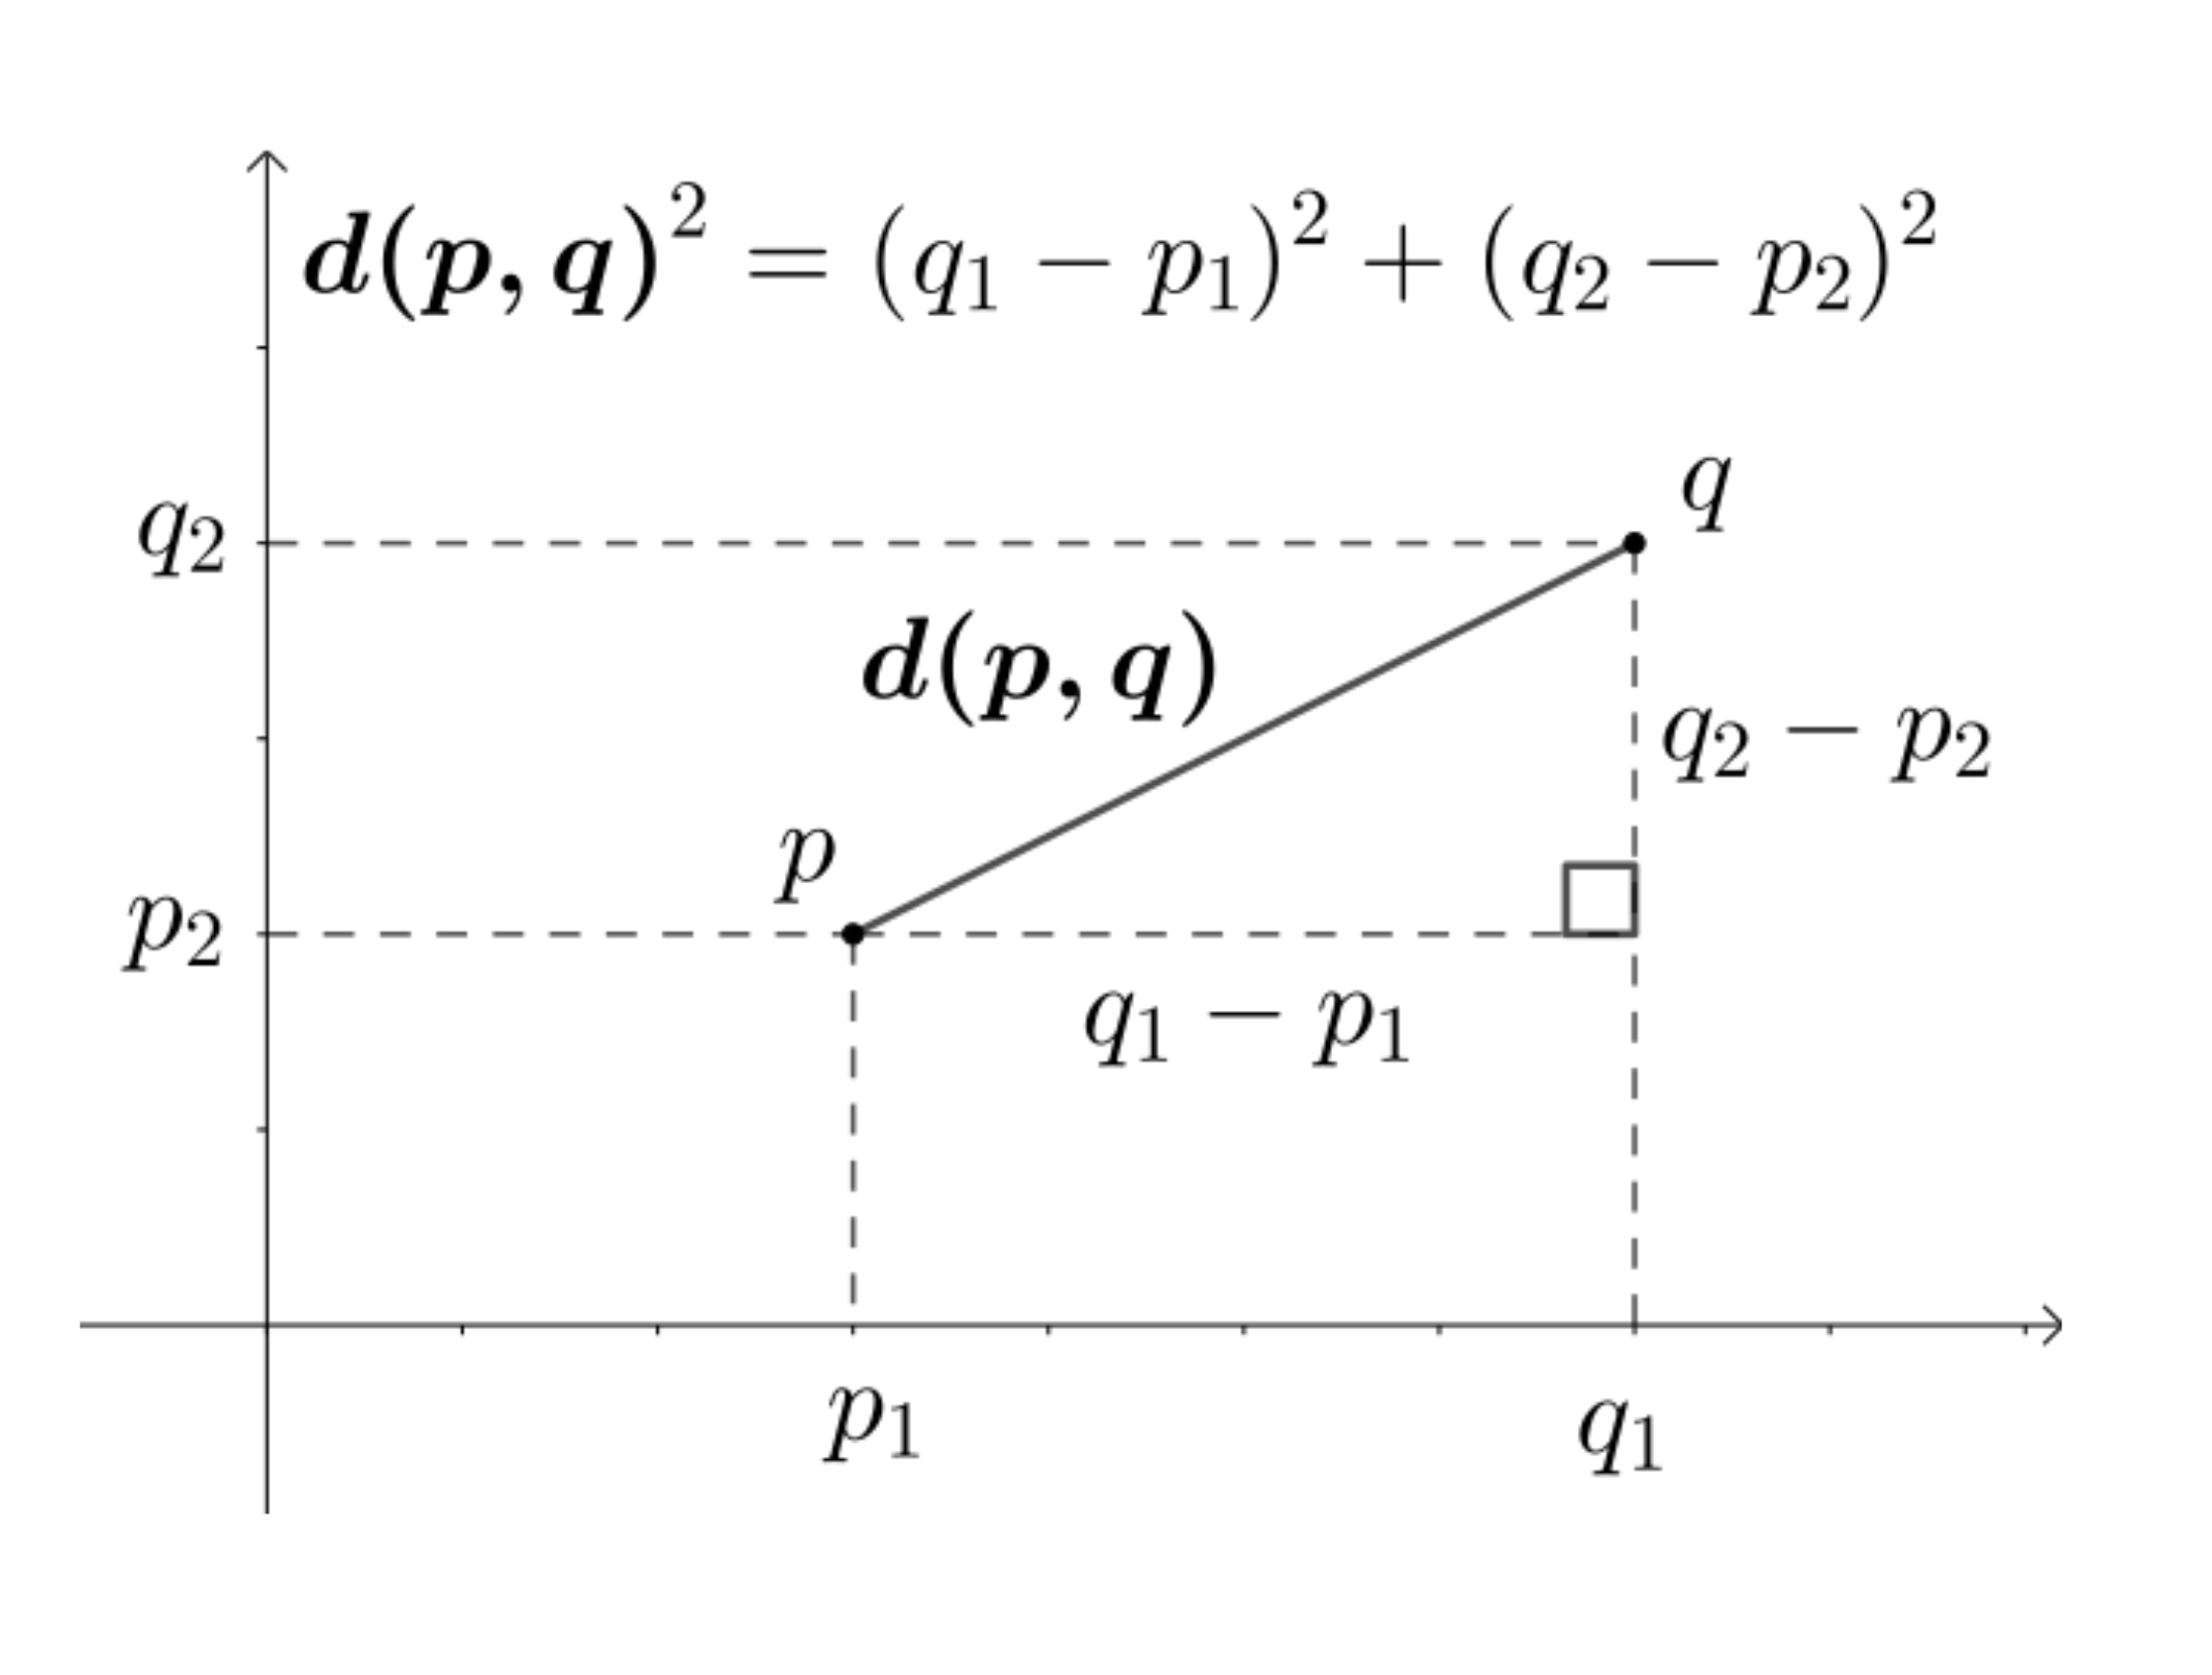
\includegraphics[width=.9\linewidth]{/home/karthik/quicklisp/local-projects/cl-dist-measure/data/pythagorean.png}
\caption{\label{fig:org36c3078}Pythagorean theorem}
\end{figure}

\section{Distance Formulas}
\label{sec:org004994f}
\subsection{One dimension}
\label{sec:org9c9bbca}
The distance between any two points on the real line is the absolute
value of the numerical difference of their coordinates. Thus if \emph{p} and
\emph{q} are two points on the real line, then the distance between them is
given by:

$$
d(p, q) = |p -q|
$$

$$
d(p, q) = \sqrt{(p-q)^2}
$$

\subsection{Two dimensions}
\label{sec:orga7cd196}
In the Euclidean plane, let point \emph{p} have Cartesian coordinates \emph{(p1,
p2)} and let point \emph{q} have coordinates \emph{(q1, q2).}\\
Then the distance between \emph{p} and \emph{q} is given by,

$$
d(p, q) = \sqrt{(q_1-p_1)^2+(q_2-p_2)^2}
$$

\subsection{Higher dimensions}
\label{sec:org8d21443}
In general, for points given by Cartersian coordinates in n-dimensional
Euclidean space, the distance is,

$$
d(p,q) = \sqrt{(p_1-q_1)^2+(p_2-q_2)^2+\dots+(p_n-q_n)^2}
$$

$$
d(p, q) = \sqrt{\sum_{i=1}^n(p_i-q_i)^2}
$$

\subsection{Disadvantages}
\label{sec:org4cd1dd1}
Euclidean distance is not scale in-varient which means that distance
computed might be skewed depending on the units of the features.
Typically, one needs to \textbf{normalize} the data before using this distance
measure.\\
Moreover, as the dimensionality increases of your data, the less useful
Euclidean distance becomes. This has to do with the curse of
dimensionality which relates to the notion that higher-dimensional space
does not act as we would, intuitively, expect from 2 or 3-dimensional
space.

\section{Cosine Similarity}
\label{sec:org6d20852}
It is a popular method for approximating how similar two vectors are.
The intuition behind cosine similarity is relatively straightforward, we
simply use the cosine of the angle between the two vectors to quantify
how similar two vectors are.\\
From trigonometry we know that the

$$
cos(0^\degree) = 1
$$

$$
cos(90^\degree) = 0 \space and \space 0 <= cos(\theta) <= 1.
$$

\begin{figure}[htbp]
\centering
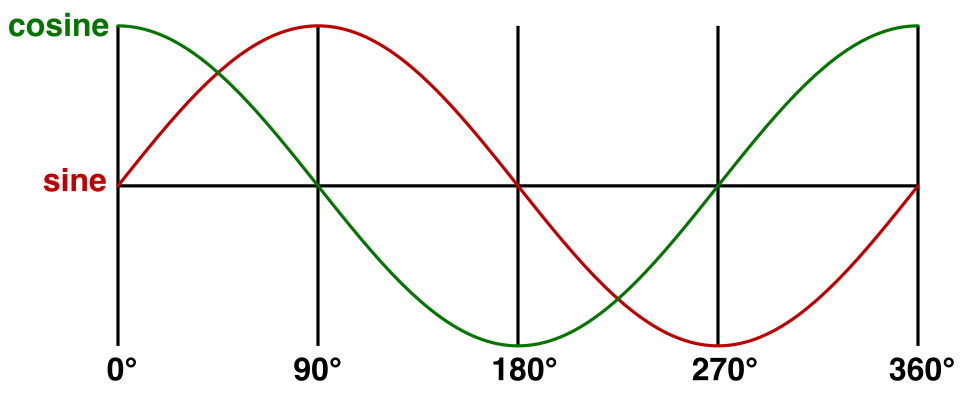
\includegraphics[width=.9\linewidth]{/home/karthik/quicklisp/local-projects/cl-dist-measure/data/sine-cosine.png}
\caption{\label{fig:org531c4fb}Sine and Cosine Wave}
\end{figure}

\begin{figure}[htbp]
\centering
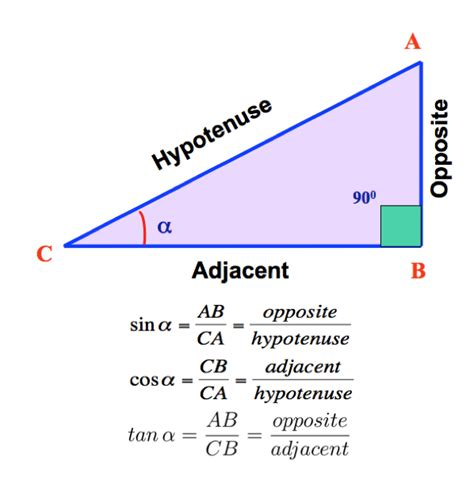
\includegraphics[width=.9\linewidth]{/home/karthik/quicklisp/local-projects/cl-dist-measure/data/cosine_sine_tan.jpeg }
\caption{\label{fig:orgdbea927}Trigonometry}
\end{figure}
The Dot Product of two Euclidean vectors** \textbf{a and} **b is defined by,

$$
a \cdot b = \|a\| \space \|b\| \space cos \theta,
$$

$$
cos(\theta) = \frac{a \cdot b}{\|a\| \space \|b\|}
$$

$$
cos(\theta) = \frac{\displaystyle\sum_{i = 1}^n A_iB_i}{\sqrt{\displaystyle\sum_{i = 1}^n A_i^2}\sqrt{\displaystyle\sum_{i = 1}^n B_i^2}},
$$

\begin{quote}
Two vectors with exactly the same orientation have a cosine similarity
of 1, whereas two vectors diametrically opposed to each other have a
similarity of -1. Note that their magnitude is not of importance as
this is a measure of orientation.
\end{quote}

\subsection{Disadvantage}
\label{sec:org41ad27f}
One main disadvantage of cosine similarity is that the magnitude of
vectors is not taken into account, merely their direction. In practice,
this means that the differences in values are not fully taken into
account. If you take a recommender system, for example, then the cosine
similarity does not take into account the difference in rating scale
between different users.

\subsection{Usage}
\label{sec:org179e488}
We use cosine similarity often when we have high-dimensional data and
when the magnitude of the vectors is not of importance. For text
analyses, this measure is quite frequently used when the data is
represented by word counts. For example, when a word occurs more
frequently in one document over another this does not necessarily mean
that one document is more related to that word.

\section{Reference}
\label{sec:org8e900d5}
\href{https://stats.stackexchange.com/questions/99171/why-is-euclidean-distance-not-a-good-metric-in-high-dimensions}{Why is Euclidean distance not a good metric in high dimensions?}
\end{document}
